\documentclass[]{article}

\usepackage{hyperref}
\usepackage{graphicx}
%opening
\title{Planetary Annihilation - The Battlemanual}
\author{Sajuukthanatoskhar}

\begin{document}

\maketitle
\begin{figure}[h]
	\centering
	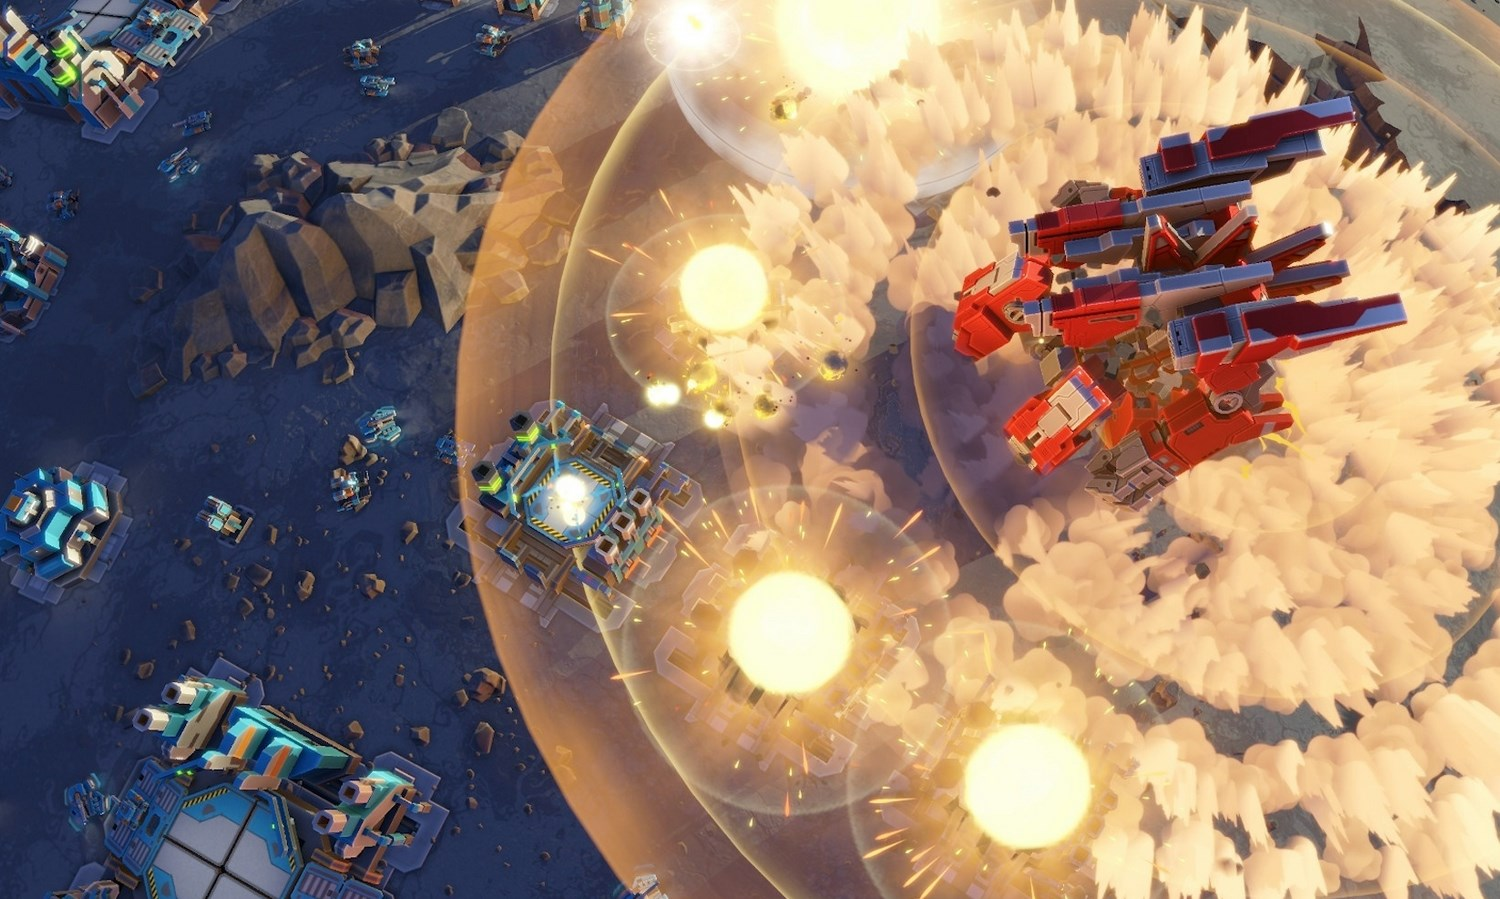
\includegraphics[width=1\linewidth]{5seQd0e}

	\label{fig:5seqd0e}
\end{figure}


\newpage
\tableofcontents
\newpage
\section{Introduction}

I am Sajuukthanatoskhar.  Some of you will know me as the toxic guy, spammer noob, butcher of new players and generally all round terrible person.  Some of you others will know me as a capable player, who carries games when I want to.  I used to play ranked and achieved \#8 in Uber for a time, but then I had to write a research paper and never went back to it.  My alignment is probably chaotic neutral.  

I have been playing PA and Titans since 2014, since part way through the Alpha.  I have been playing Total Annihilation (and TA:Spring) since 2007, and played Supreme Commander.  The play styles are slightly different from each other but I enjoy these games far more than say Starcraft or Civilisation, although I am a fan of Sid Meier's Alpha Centauri, Hearts of Iron 3/4, Homeworld and Age of Wonders Shadow Magic.  

I also play EVE Online with my alliance TEST Alliance Please Ignore as a diplomat, Fleet Commander and alliance corp CEO.  


\section{Acknowledgements}

My thanks to all the players that have fought me, new and veteran.  Some of you put up a spectacular fight that make me rethink how to do things.  

Uber Entertainment for having made a pretty cool game that is, in my opinion, rather underrated like many Annihilation titles in the past.  

Sorian for having good one on one conversations on TEST Alliance mumble back in 2014 about the bloody pathfinding.  You disappeared from the alliance, but not from my heart.

\section{This strategy guide and who it is for}

This battleguide will not walk you through how the basics of the game work.  I wish to only give out the secrets of the brotherhood of Uber players and some of my thoughts on how things work and what others should be aware of.  

Sometimes I will mention things that are seemingly obvious, but I once read a book (amazing, I know) called Sophie's World and in the book, the point where the obvious things in this world are still worthy of investigation was raised.  

\subsection{Assumptions}

I will assume you have read or played enough to know every unit in the game to an extent they are like the lost sibling of your family.  Like a sibling however, they have secrets and they are on the palobby website.  I will make references to this website for any technical point.  It is located \hyperref{https://palobby.com/units/?version=titans}{}{name}{here}.  I won't refer to Legion as it is not officially part of the game yet (as in it needs to be not a mod that must be downloaded everytime you join a server)

What I will touch on will be orbital mechanics as this is the most unobvious set of mechanics to most players.  In addition, I will talk about \textbf{teleports}, how factories don't use their full metal use listed on the box for a build.    

\subsection{For the new players}

This guide is not really meant for you (but you are free to read through it).  But here's some words of advice.  

You expand, you build more factories, you kill your opponent.  You need to have a whole bunch of different tactics up your sleeve, recognise possible situations and be implement plans on the fly.  You need to have a lot of self awareness and the only way to get better is to play multiplayer.
  

\subsubsection{When you die}  

When you die, review what happened.  It is so vital.  Stay around and ask the player how they did it, I'm sure their ego will drive them to explain how they rushed 30 boombots around your dox and got to your commander.    


\subsection{A word on world ending devices}

Yes, it is in the name of the game, but planetary annihilation is one of the final steps you take to gain victory.  They are extremely metal hungry and fragile to any form of aggression.  Personally, I don't like ragging, lasering or hitting planets.  I might need it for later.  The circumstances for actually doing so involve the impossibility of a space based invasion (due to the planet's economy), it is far more cost effective to then build a ragnarok/catalyst/halley.  

Just remember, PA:Titans is about killing the commander in some shape or form.  As a new player, you won't know everyone in the community and because of that, when you see a commander (barring multiperson FFAs, you might want to keep someone alive to be a meatshield (diplomatic or otherwise) against a far more powerful player), you kill them if you can, doesn't matter how glorious the kill could be, you just do it.  

\begin{figure}[h]
	\centering
	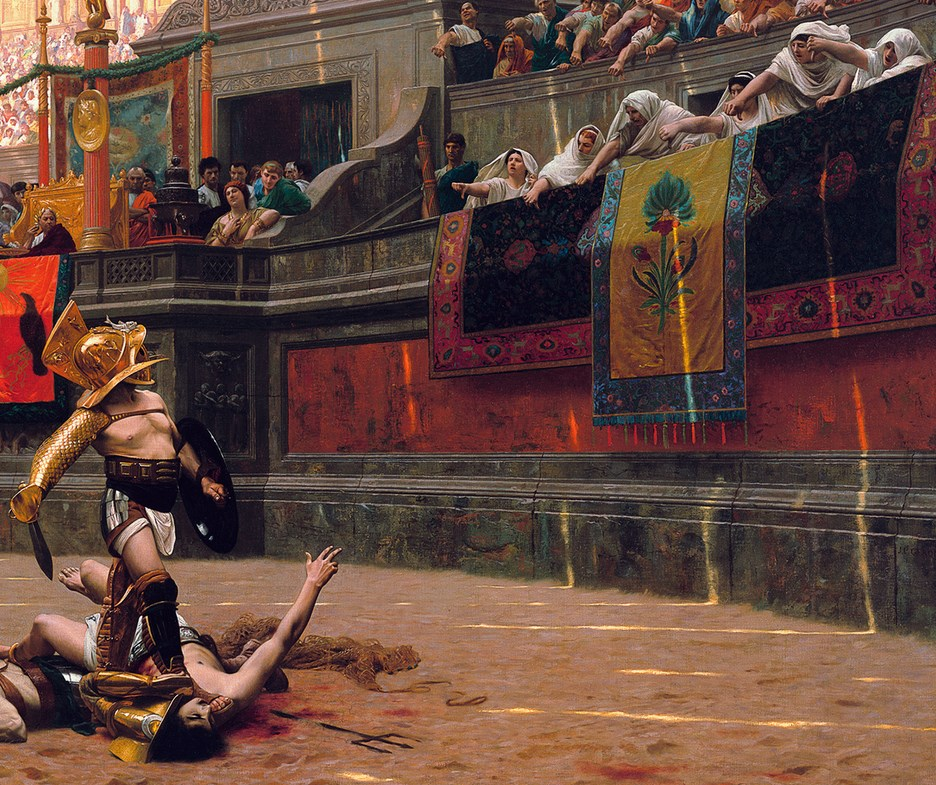
\includegraphics[width=\linewidth]{NtpMQAd}
	\caption{PA:Titans - No mercy whatsoever.}
	\label{fig:ntpmqad}
\end{figure}


\newpage
\newpage
\section{Bounty}

Planetary Annihilation Vanilla players, you miss out on this gem of a game option.  In Titans, this is used to sometimes 'equalise' FFAs.  In more cases than not, unless the bounty value is set to 0.01x or something disappointing, it does the following
\begin{itemize}
	\item Make competent players turn into absolute savages and is equivalent (if there is such one) of turning them from Queller Uber to Skynet difficulty
	\item Makes weak players look like giant pinadas
	\item Should a competent player (like some ranked Uber players) get a bounty, they ascend to a status that ranges from a Cheating Sorian++ Adaptive AI from Supreme Commander to godhood.  Note, they aren't actually cheating
	\item Weak players who get bounties grow massive targets on their backs from more skilled players as the metal produced puts them at odds with these players.  
\end{itemize}

\textbf{Author's Note: }For me, getting bounty is probably one of the sweetest things to get in a multiplayer game of any kind.  There is nothing more overpowering than this concept and should never be turned on.  Free For Alls are bloody and people die because they made bad decisions (sometimes to kill another player and suddenly having no army, to the joy of their second neighbhor).  Having said that, I don't mind if it gets turned on.  

\begin{figure}[h]
	\centering
	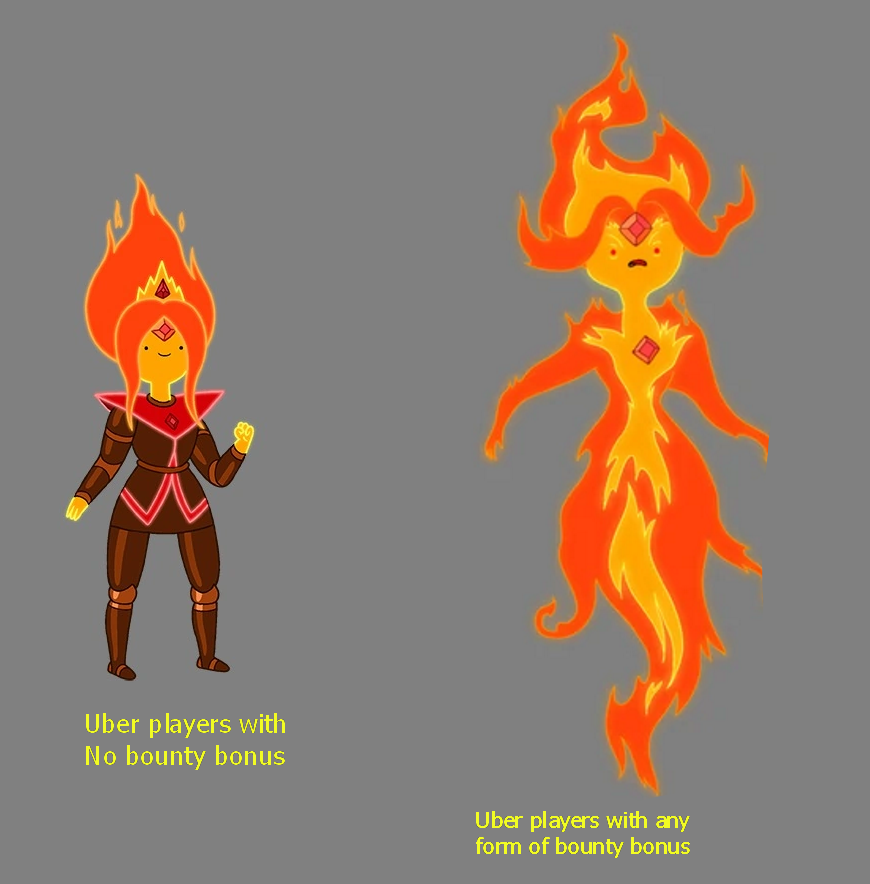
\includegraphics[width=0.5\linewidth]{cOkgxlH}
	\caption{This is what happens when Uber players get a bounty bonus. The same set of pictures (from Adventure Time btw) could be used to describe the level of aggressiveness of an uber player up on knowing that the game they are in is a bounty game.}
	\label{fig:cokgxlh}
\end{figure}




\newpage 
\section{Attention Warfare}\label{sec:attention-warfare}

There are three resources in Planetary Annihilation.  Metal, Energy and Attention.  

Your attention to the whole game as a whole is a resource that is, unlike Metal and Energy, finite. Your attention needs to be divided up carefully or you will lose a section of your war against a player purely you weren't thinking about it.  This gets incredibly hard when you have to fight across multiple planets simultaneously (however it is rather epic).  

Attention warfare is a thing and if you can willfully manipulate your opponents attention, then that is far more powerful than killing his economy as it leads to the destruction of that economy.  

\subsection{Choosing what planets should do what}  

Some planets are better to have lines of factories on it than others.  Typically, Moons are the best for this whilst Metal Planets are the worst (due to them being divided in three).  Making a decision can simplify your production side of things, especially if units go to a single point (such as a teleport).  This allows you to only have to worry about any orbital to land invasions.  
 
\newpage
\section{Pre-Game Decisions define your entire game}

Many games have multiple planets, multiple starts, multiple possibilities.  

In team games, it is essential to communicate where you are starting, to optimise your game.  Sure, PA is about fun, but it is a thinking person's game and position is everything.  

\subsection{Red vs Blue Team Games}

In most games, you have one team vs a second team and you fight it out.  You need to place yourselves in a way that will win you the game.  

In this typical setup, you might have multiple planets and games are decided in the starting stage of the game where players choose where to go.  

\subsubsection{Starting on one planet}

Is not good if there are others to start on.  Players might quickly kill an enemy on that planet but after that, metal will be split by the players on the planet and if there is limited metal, it can be hard to assemble an army.  

Spreading out is scary to new players and lots of encouragement must be given to make them start solo on a planet.  There are reasons for this

\begin{itemize}
	\item Maximum Possible Expansion - starting on as many planets as possible allows you to grab as much metal as possible across your whole team.  This is especially true on shared matches.  
	\item Keeping the enemy at bay - If one player per enemy is maintained, then there is no possibility for a rapidly expanding enemy to swoop in with an advanced army and save the day.  
\end{itemize}

\subsubsection{Lane games}

These are maps with one planet that pits you in a lane against another player, you have no choice, no say.  The players have their one and only start spot and that is that.  


\subsection{NvNvN... Team games}

In multiple team games, the starting has a lot more decisions to make.  You may choose to start on a single planet with your allies, and rely on the other teams spawning on the other planet, giving you free reign over your starting planet(s).  

A small discussion might be needed, maybe it is good to split yourselves up or start on the same planet.   

\subsection{Individual Planet choices}

Choosing a planet based on metal is sometimes not the best strategy.  A planet might have lots of metal and thus is a popular choice.  You might have to fight out against all other players.  



\newpage
\section{Planets with high amounts of doodads/CSG}

These planets are horrific for unit pathfinding.  Flatly said.  Veterans will hate dealing with this and because of it, makes for an unsuitable location for mass factory layouts, unlike a moon.  The one way to get aroudn it is to waypoint teleporters. However, these are easier to defend using holkins and artillery being placed behind the CSG, using them as natural barriers to enemy encroachment.  
\newpage
\section{Gas Planets}


Gas planets are a treasure trove for resources but are simultaneously extremely vulnerable to attack, mostly due to the way jigs explode upon death.  

A game can be decided with it.  

It should be said that a space fabricator travels slowly across a planet, indeed perhaps one of the slowest fabricators.  It takes time for jigs to be built.  It must be important to remember that they must travel a certain distance to ensure jigs are built outside of their death explosion radius.

As mentioned in \ref{sec:losing-gas}, losing gas is a terrible to happen.  Players will resign, disconnect and call you all sorts of names, demonstrating the importance it was to their battle plans.  

If a player has  control of gas and land, it is highly adviseable to either attack the land or gas planet with a pure focus.  Many players will build on gas, get alot of resources and given time, build an impregnable defense with many nuclear silos, a massive army or both.  

Not dealing with this massive threat early enough can jeopardise your entire game.  

\newpage
\section{Orbital Mechanics}

Planetary Annihilation was designed around the four combat layers we love.  The most mysterious is the orbital.  Hardly used in \textbf{lane} maps, the units can be incredibly metal intensive, the \textbf{fabricators} are expensive to run with power but if you manage to control a gas planet and its resources, you are both extremely powerful and at the same time, very weak.  

I am not going to write about how you established multiple Cloud City's and then deleted 7 players, including 3 of your allies with nukes you conjured up in 20 seconds with 100 \textbf{t2} \textbf{fab}s.  There are certain parts of orbital mechanics that need to be discussed prior to diving into the rest of the land, sea, air strategies.  

\subsection{Astreus}

Want to move land and air units off of the planet?  Great!  Want to do it painfully with a lot of mouse clicks?  Then you, my good sir/madam, have come to the right unit. 

The Astreus is an excellent transport unit to tell your enemies and allies alot of things.  

\begin{itemize}
	\item That you are about to leave the planet you are on
	\item That your commander is about to have its hitpoints reduced to 1\% and is now hittable by t1 fighters.
	\item That, personally, you are a coward and don't trust your allies to help you out.  
	
\end{itemize}

\subsubsection{The pullout maneuver}

That's right.  Just like in real life, the pull out maneuver done by many young commanders is not only unsuccessful, it also generates alot of tears and questioning if the other player cheated.  Rarely, if seen by a competent player, are passed unharmed and unscathed.  This is the number one strategy that can kill a commander faster than the self destruct button or 31 boombots with no dgun defense.  

\paragraph{What is it, Sajuuk}

Ok.  So the battle goes like this - 

\begin{enumerate}
	\item Player A is fighting Player B, no one else is there, no one is involved, no one cares about you two
	\item Player A is winning, Player B senses it and seeks to survive via getting to a second planet
	\item Player A maybe has the metal advantage and should have scouted your base a little
	\item Player B builds an Orbital launcher (land one), and then builds Astreus. Suddenly, everyone can see the glorious orbital unit, all players are notified of your existence across the map and they can now double click your name/icon in the top left where in most cases, where your commander is.  \textbf{Caveat:} Planetary Annihilation Classic players, this is relevant if you have power and an orbital radar, expansion players disregard
	\item Player A is not stupid, realises they are winning and wants the delicious bounty (Again, PA Classic players disregard)  from the kill of the commander or perhaps, the glory of a pull out Astreus commander kill.  They start building an air factory, maybe a few and in very short notice.  
	\item if it is an avenger space fighter that is built first, it buys the player some time before the next unit is built and amass a viable airforce.  If it is an astreus, maybe not so much.  It should be said, if Player A scouted the base and saw said orbital launcher, they will have an airforce ready incase of this event happening.  
	\item Player B goes to pick up their commander, Player A sends all ground forces if possible to follow where the commander is, it could be quite far for the astreus to go.  The airforce of AA fighters also follow.  
	\item Player B's astreus swoops down to pick up the commander.  It reaches the commander and is in the clutches of the transport and... OH NO IT DIED.  
	\item Player A has intercepted the Astreus at the right time and 2 shot KO's the transport with the commander, losing his entire airforce, killing an enemy commander and no commander metal to reclaim (this is debateably sad). 
\end{enumerate}

Sometimes, it doesn't go like this and the commander actually gets off planet safely or the Astreus is a decoy, but I rarely have seen this and the aforementioned scenario is the one most likely to happen.  

\subparagraph{Special submove}

The commander escapes and gets to their target destination.  They attempts to land their astreus and then gets killed by an enemy airforce anticipating their arrival.  This is also ok, but bounty goes to the player that kills them.  However, they don't get the commander metal as it, like on the first planet, fizzles into $E=mc^2$.  No, you can't harvest that either.  

\paragraph{Summary}

Your thoughtful but soon to be defeated opponent wants out, goes with the Astreus route, tries to pick up commander, you come in with an airforce and kill him and his astreus as it is in the \textbf{AIR} Layer and not some special air/space/invincible layer.  The commander dies, you get the bounty.  

\paragraph{What should've been done}

Space is the correct way to leave the planet.  However, you should leave using an orbital fabricator.  The combined metal cost of the two teleport gates and orbital fabricator is around 3400 metal, include the factory it is 5200 metal.  This is expensive and you could've built a t2 lab instead but if you are losing already, you might as well give it a go.  If you can't get it up in time, then you didn't have enough to rebuild and move your economy to the next planet any way and should probably resign yourself to your fate.  

\subparagraph{Exception: Water planets}

Water planets are the only exception to this rule.  You can't build a teleport on the ocean in PA:T or Vanilla.  Astreus are the only way to pluck yourself from the world that is \textbf{Kamino}. 

Make sure you build lots of aircraft and torpedo launchers to counter Narwhals, which have AA capacity.  \textbf{Bug Alert:} From memory, Narwhals might have Anti-air capability but do not (as of the date of this book) have the capability to shoot down an Astreus.  Lucky you.  

\subsection{'Teleporting' Space units}

This little maneuver of space units in general is the ability for them to be moved to a planet and then moved back to another place, despite their original location before, and be somewhere completely remote.  These places could be:

\begin{itemize}
	\item Halfway around the planet
	\item On top of your commander!
	\item Next to your commander and building a gate!!
	\item Spreading radar all over the planet before doing step 2.  With Ion Cannons.  
\end{itemize}

Of course, the time of travel is dictated by a few factors, mostly distance between planets and if I am not mistaken, how much space travel they have done recently.  

\subsection{Tech 1 Radar Satellites}

These are okay for mobile radar stations with extended scouting coverage.  The one problem is that they can't see mines.  This is okay and would be overpowered, in my opinion.  They are very cheap for what they can do but require a modest sum of energy for any tech 1 unit or building.  They are also incredibly tanky for some reason with the 4th most amount of HP out of any of the orbital units.  

\subsection{Defense against the Mongolian Ion Cannon horde}

In most cases, the generation of these hordes means they have a gas giant and you are on the losing foot.  It is impossible to defend against 50+ Ion Cannons landing ontop of your commander, save that you sent a nuke to hit your commander at precisely the right time all these ion cannons land, but it takes two shots to finish you off.  

\textbf{Battleships:} The Omega battleship is a very expensive counter to the Ion Cannon swarm and could be dealt with a detachment of Artemis railguns, which of course counter the short range guns of the Omega.  The Omega is no flak cannon of the orbital layer, only the nuke can have that claim.  Considering the cost of the Omega (14000 metal) vs the cost of one nuke (Silo is 14400 metal, Nuke is 30000 metal), this is a debateable defense and is conjecture at this point.  

The alternative strategy is to fight the player with space first, take control of gas by preventing others from building on it and not building on it yourself (to minimise your threat footprint)

\subsection{Stealthy Unit Cannons}
\label{sec:stealthyucannons} 
Whilst not a space unit, the Unit Cannon fires projectiles that can be seen across the map, show your color and where there are going and coming from.  However, it does not tell players, who are not watching the interplanetary layer, of what is going on.  There are no notifications.  There are no signals.  There is nothing.  It is the closest thing to a stealth move in the game and is relatively cheap for the price you need to pay versus the reward of moving to another (possibly uninhabited) planet.  

The cost of at least one unit capable of build a teleport and a unit cannon is 10000 metal.  It requires 4800 metal for a t2 factory and a 2000 for a t2 fabber.  This means you need roughly 22000 metal to pull this off and is hard in early game.  However, if no one else is expanding by space, then this is the way to go.  It is recommended to do this if you are alone on the planet and can reach \textbf{peak planet metal} without resistance.  

Every other space unit, announces your presence, double clicking the top left commander icon will center the camera on that unit and thus the planet you are most likely on.   

\newpage
\section{Teleports}

Teleports, as you should know, are the mainstay for fast reinforcement on none lane maps, tricky maneuvers and sending your own troops through to remote locations

But they are also extremely good at the following:
\begin{itemize}
	\item Sending your enemy's land units
	\item Finding out which planet you sent your commander too, prompting a precision invasion response as if you never left the planet.  
	\item Following point 1, killing your own commander if you have sent it through and left it hanging on the other side.  Mostly using boombots.  Just remember, teleporters have a default waypoint and it as at the front door.  It's very sad but its up to you, the coward that you are, to fix this and move your commander away.  Or you could just turn off your teleport.  
\end{itemize}

The strategic advantage of all these are not lost to competent players of PA.  

\newpage
\section{Nuclear Missiles}

As a veteran TA player, a nuclear missile going from silo to unprotected base means an imminent end to a game.  In PA, its less so.  These missiles are slow, can't one shot kill Titans (maybe Zeus, not tried)  and very expensive (30000 metal).  The silo itself is 14400 metal.  I always see new players waste so much metal into these things.  There are far better things to spend that metal on.  

In reference to a future chapter, the 2Mex1Fac strategy used in early game for tanks uses 5 Ants, 1 Inferno, 1 Spinner.  This is a total of 1125 metal per run of these.  You can make 39 of these groups instead, which will, in most cases, do more damage.  For 1 Gile and 1 Bluehawk, you can make 22 of each of these and have a very nasty battlegroup that will kill most T2 tank armies.  The only real use of a nuke silo is purely to have something waste metal into or have a very powerful defense against space threats.  


\newpage




\section{Space Invasion Strategies}

I normally only do these particular space invasion strategies.  There are some conditions why and when I would use each particular one.  I go into the reasoning for each one in each section

\subsection{Scouting}

Just remember, you can always scout using a Pheonix fighter or a radar satellite.  


\subsection{Tier 1 : Single Space Fabricator}

The easiest way of getting across space is by fabricator.  Minimum cost is 1800 metal for the factory, then 1800 metal for the fabricator.  

\subsection{Tier 2 : Many Space Fabricators}

The logical next step up.  You lost a single space fab to an avenger, or the gate will be built too slow to resist counter attacks?  You build many more space fabricators.  

\subsection{Tier 3 : Unit Cannon with combat fabricators}

The unit cannon can be used to \textbf{stealthily see \ref{sec:stealthyucannons}} get across space without causing notifications.  It is much faster than any space unit.  Combat fabricators (Mend or Stitch) are produceable relatively quickly and build extremely fast.  An invasion teleport can be built within seconds if metal and energy available. 

\subsection{Tier 4 : Helios}

This is a lesser version of a teleporter in my mind, as it doesn't have an exit waypoint that you can set and units will just sit as soon as they appear.  

\subsection{Tier 5 : Nuke + Helios or Unit Cannon}

This is a combination of using a nuke or two to clear out an area full of catapults or some other nasties on the ground so you can get troops there.  Expensive.  looking at around 75k metal for Nuke and Helios.  



\subsection{Tier 6: Apocalypse - Multiple nukes, Pheonix Invasion, Multiple Helii Titans and Unit cannons}

At this point, you are desperate enough to build nukes to clear the area that you want to drop to start your invasion.  

\begin{itemize}
	\item The Nukes clear space
	\item The Phoenixs keep the area clear from air fabricators and Zeus titans that could be ready to defend.  
	\item One gate with an army streaming through is not enough, you need many gates with the same number of Helios titans to do the same
	\item Unit cannons maybe, just to be sure.  
	\item Manhattans can be dropped here via a delivery Helios to help clear titans and unit blobs that may be there, but I have never done this.
\end{itemize}

This can be hard to counter but if it is, do not lose hope.  


\newpage
\section{General Strategies}


\subsection{Word of warning}
The following two sections describe set battle startup strategies.  These should not be dogmatically followed but taken as a guide.  New players are very welcome to play with these setups.  When you have a certain feel for unit compositions and what is needed, you don't need to follow them so strictly. 



\subsection{2Mex1TankFac1AssFab}


Personally, my favourite strategy and normally my starting strategy since Nov 2019.  It is simple, you build a factory for every two metal extractor with an assisting fabricator.  Most of the time this is a tank factory.  The assist fabricator can be used to build a building prior to assisting (its up to the commander and for me, normally its a radar or a metal extractor).

The end result is a lot of units being produced.  Is it worth it though?    
\begin{figure}[h]
	\centering
	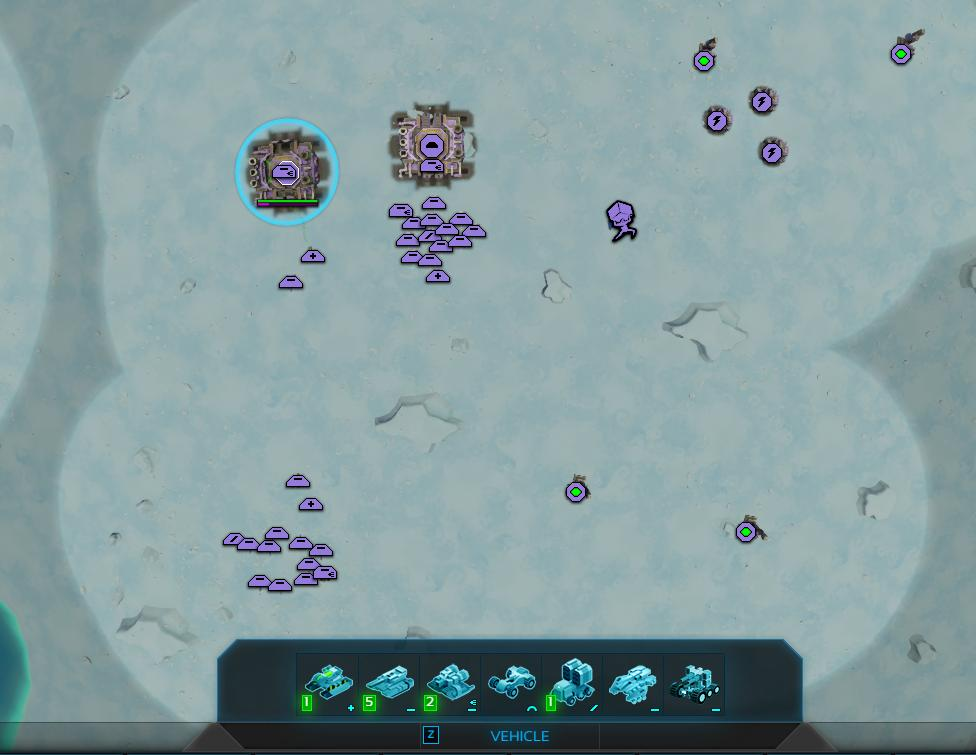
\includegraphics[width=0.7\linewidth]{SBi860w}
	\caption{The 2Mex1TankFacAssFab build ratio is shown at the bottom. Make sure your factories have their queues set to looped. You are always building units.}
	\label{fig:SBi860w}
\end{figure}

\subsubsection{Why the extra build power from fabs?}
This increases the build power of the factory by 11 metal/s for land, 8 metal/s for bots and 9 metal/s for air (all t1).  This is a 73\% faster build rate when the recovery time of a factory is not taken into account.  With the recovery time, a land factory (the one with the longest recovery time of around 4 seconds, 3 for bot factories and 2 for air, t1 and t2), will have an increase of 56\% productivity.  This means there are diminuitive returns.  

With the use of the first fabber and tank factory, the utilisation of metal is higher (15.78 m/s) than the collection rate of the metal extractors (14 metal/s).  Normally this is much lower, see \ref{sec:real-costs-of-production}.   
\subsubsection{Evolving into mid game}

The strategy works into mid game as a lot of fabbers will be available for utilisation.  An emergency shift to t2 is possible should the need arise.  All fabbers at that point should be put on the t2 factory.  The strategy tends to just devolve into building a shit ton of 
%4 sec land
%3 sec bot
%2 sec Air





%\subsection{1Fab6+1dox_Per_Fac}

This is a second 



\subsection{Dox Swarm Build}

Again another simple build, a ratio of 1 bot fabricator to 5 dox is needed, with the fab being built first. 




The economy ratio for this is 1 metal extractor and 1 power generator for every factory.  No assisting the factory.  Use the fabs to expand and the dox to attack and scout, repeat ad nauseum.  Soon you will have a lot of dox and can now either push your commander into the enemy base and pin him down or even out right kill him, just watch out for grenadiers or shellers (don't push your commander into a base full of shellers) who will be aiming for your comm but will hit your dox, exactly what you dont want to have happen.  See \ref{commpush} for more information.  

\textbf{Wait? Don't grenadiers fire ahead of a moving unit? WHAT! }:  Indeed they do, the pushing of the commander is done at the speed of the dox, the commander is still going its original speed (but he gets pushed), the grenadiers use the commander speed value, otherwise the mathematics for instantaneous velocity would have to be calculated for everything (overloading the servers).


\begin{figure}[h]
	\centering
	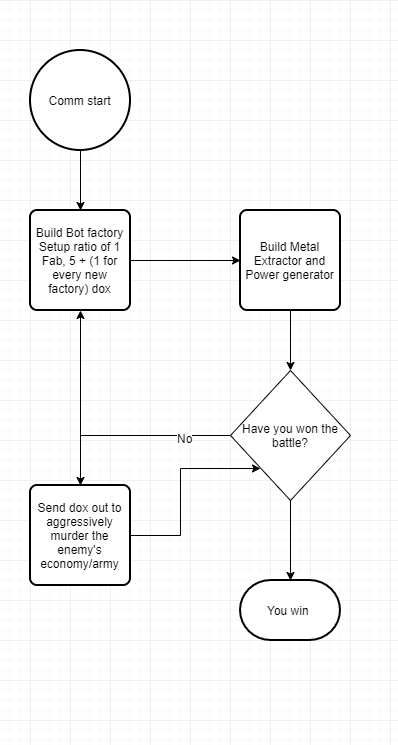
\includegraphics[width=0.5\linewidth]{tZQ7AcE}
	\caption{The general idea for this strategy is outlined here. Be aware of the weakness of dox blobs}
	\label{fig:tzq7ace}
\end{figure}

\subsection{Air starts}


Why?  

More seriously, many new players start out with air, its fast, its planes and its plain fast.  Cool.  Not so cool are the ever watchful veterans who will kill those air-fabs, then pin \ref{subsec:pinning} that player down as they have no fabs left to expand with.  Air fabs with fighter support provide that much more protection (fighters still fire automatically at air fabs as priority target so you need to intercept fighters yourself).  

Air is ok for scouting, but it means you had to have build a factory to do so and in the beginning of a game, that's time that you have to figure out how to get back.  



\subsection{Real costs of production}\label{sec:real-costs-of-production}
All factories use a certain amount of resources when in use.  However, they have a delay between builds and it is worth knowing this as a concept:  Unassisted fabs do not produce at their advertised rates when applying this average.  The gap is the Unit Build Delay (my term).  

\begin{table}[!h]
	\begin{tabular}{|l|l|l|l|l|l|l|}
		\hline
		\multicolumn{1}{|c|}{Factory} & Unit & \begin{tabular}[c]{@{}l@{}}Metal \\ \\ Cost\end{tabular} & \begin{tabular}[c]{@{}l@{}}Time \\ to \\ Build\end{tabular} & \begin{tabular}[c]{@{}l@{}}Cost \\ (metal/energy)\\ /second\end{tabular} & \begin{tabular}[c]{@{}l@{}}Unit \\ \\ Build \\ \\ Delay\end{tabular} & \begin{tabular}[c]{@{}l@{}}Actual Cost \\ \\ (metal/energy)/second\\ with no fab assist\end{tabular} \\ \hline
		Tank & Ant & 150 & 10 & (15/675)/s & 4 & (10.7/481.5)/s \\ \hline
		Tank & Inferno & 225 & 15 & (15/675)/s & 4 & (11.842/532)/s \\ \hline
		Tank & Spinner & 150 & 10 & (15/675)/s & 4 & (10.7/481.5)/s \\ \hline
		Bot & Dox & 45 & 3 & (15/675)/s & 3 & (6.428/289)/s \\ \hline
		Bot & Stitch & 250 & 16 & (15/675)/s & 3 & (12.5/562.5)/s \\ \hline
		Bot & Spark & 105 & 7 & (15/675)/s & 3 & (10.5/472.5)/s \\ \hline
	\end{tabular}
\caption{Real costs of production on some basic ground units, the longer the build time, the more metal is needed per second}
\end{table}

It is worth pointing this out to know that you can get away with having more factories than your economy can seemingly allow.  

\newpage
\subsection{Pinning}
\label{subsec:pinning}

Map control is essential to expand your economy, to get more industrial capacity and to ultimately win.  But map control doesn't mean putting a tank on EVERY metal spot cluster.  Just remember that you have to win the game against your opponent, not build a city, meaning that in a situation where you have all the metal clusters in the world to control, you only need to control the ones your enemy covets (So profound!).  

This means you have to do the following:

\begin{enumerate}
	\item Scout the enemy's base
	\item Find out what factory they have built
	\begin{itemize}
		\item Tank factories are slow to expand, consuming alot of metal.  Dox or boombots are great at killing these.  
		\item Air factories consume alot of energy (through fabbers).  The fabbers are one shot killable with fighters.  Counter with fighters and kill as fast as possible.  Tanks with AA can also be used, but you can't chase the airfabs around the map.  
		\item Bot factories produce a lot of cheap, fast units.  Tanks counter offensive bot movements and can one shot kill botfabs.  
		\item If they have no factory, this is made incredibly easy
	\end{itemize}
	\item Whilst you control your enemy's metal, you can expand as fast as you like, however, the enemy will be building units or an advanced factory in order to break, what i call, a pinning move.  
	


	
\end{enumerate}
	Pinning is extremely dangerous for the player pinned.  With no further metal to expand to, every bit is now essential.  if you are pinned, death is imminent and breakout is the only way.  if you cannot breakout, you will need to either resign, escape the planet if feasible, hard counter with what you have or have an ally bear down on that opponent (taking away whatever attention your ally is putting on their enemy).  

\subsection{Sneaky Boombot snipe}

Boombots are very blind but kill non-swarm units very easily.  

For attackers 

\begin{itemize}
	\item Use a scout plane
	\item Need at least 35 boombots to kill a commander that doesn't use an Ubercannon
	\item More if he does
	\item Dox or Slammers will wreck your attack, add 10 boombots for each dox/slammer
\end{itemize}

\subsection{Direct Frontal Assault}

This is a numbers game of how much units you have vs what the enemy has.  Most DFA's are pointless if you have no idea what you are going into or why you are doing it. 

\subsubsection{Walls} 

Putting up walls against a DFA and putting units as well as combat fabricators for repair behind that wall is very effective against anything.  Lobbing or air units are the only threat in this scenario.  Titans and most advanced units will go through a wall with ease.  

\subsubsection{Who wins, takes all the wreckage}

Titans players will know that units will leave wreckage and the one that controls the field, gets to reuse that metal by reclaim it.  It is in your best interest to reclaim metal whilst you are fighting, this can be done using fabs or combat fab bots.  


\subsection{Use of terrain}

Using the terrain to put a stop gap between the enemy and you whilst killing their base is extremely effective, if it is possible.  

Only the longest range units and buildings with lobbing weapons (Grenadier, Bluehawk, Sheller, Pelter, Lob, Catapult, Holkins\textbf{(min range)})) can deal with elevation differences effectively.  Direct fire weapons will have a tough time but can be possible. 


\subsection{T1 Tanks : The inferno}

The inferno/flame tank is extremely useful as a meatshield.  When combined with a combat fabricator from the t1 bot factory, ants or dox can sit behind the inferno wall and fire with impunity.  Whilst they are shooting, the infernos will soak damage and if they come in contact with a unit, incinerate it (flame vs metal, must be very hot).

The Vanguard T2 Tank also can function like this and can in effect, 

\textbf{Author's Note: } Actually there is a nice mod in the PA community that turns the flame blue and makes it more like lightening.  Looks super cool.  


\subsection{T2 Tanks: The Leveller}

Many times I have seen the leveller get used.  It is probably one of the most popular t2 units used and for good reason - it is hardy and can kill a commander before a commander can kill it.  

Two important things regarding the leveller must be considered when taking it into battle.
 
\begin{figure}
	\centering
	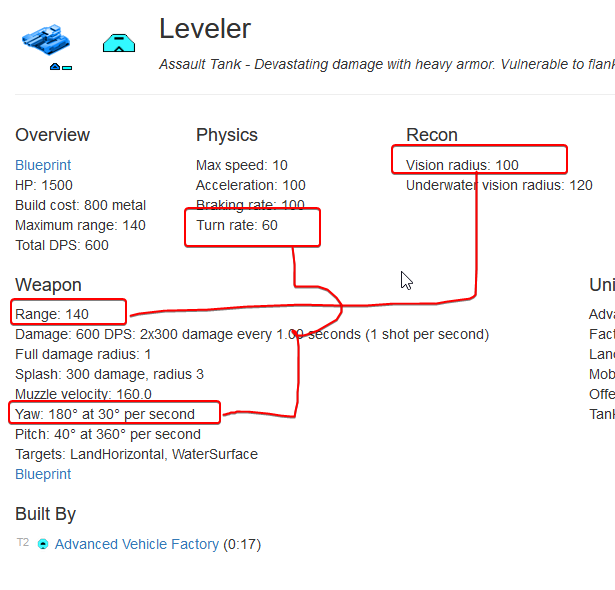
\includegraphics[width=\linewidth]{zp9bTfg}
	\caption{Aspects of the Leveller to watch out for}
	\label{fig:zp9btfg}
\end{figure}
\subsubsection{Vision Radius}

They need scouts.  Pure and simply, the lack of radar or scouts means that they can be taken on by an Ant at the same range, albeit will die very quickly.  

If the leveller had a scout to extend its sight, it will be capable of firing earlier.  How much earlier?  4 seconds earlier - this is because it moves 10 length units per second, fires once per second and there is a 40 length unit difference between maximum sight and turret range.  Given the speed of an ant would probably be going directly toward a leveller, this would be shortened to two seconds.  

In short, use a scout.  

\subsubsection{HOLD THE LINE THERE BUDDY}
Look at the turret turn rate of the leveller.  It is half the actual turn rate of the whole tank.  This means that the turret will turn roughly with the leveller should it do a really tight turn, which happens alot when the player seeks to kite an enemy player.  This is, by the way, a valid strategy but many do it whilst their levellers are under fire, losing many to when they should've done is just kept the tanks there or turned them around.  The situation is so bad that its worse than not having a scout with the leveller.  So, if you are facing overwhelming odds and can't do anything about it, leave the levellers there to kill as much as they can. 

\subsection{Other T2 Tanks}

I only want to really talk about the main combat tanks here.  Manhattans and Storms have their own obvious uses but don't have anything worth talking about here in respect to what they do.  
\subsubsection{Shellers}

Shellers are great for dealing with all long range bots and actually outrange them.  Their shells have splash damage and can kite effectively.  They can also deal with base defenses quite effectively.  

They are incredibly vulnerable to air attack,  

\subsubsection{Vanguards}

These are moving walls of plasma ball death.  They can soak up a lot of damage and are perfect as a screening force for any other unit type, including T1 units.  It should be noted that Inferno tanks are better at dealing with boombots than Vanguards.  
 
\subsection{T2 Bots}




\subsubsection{Gile Sniper Bots}

Giles are amazing anti-T2 units.  They are only vulnerable to mass unit blobs, bad decisions and tight spots.  They are slow to turn their weapon, alot of care must be taken to ensure maximum effectiveness.  Their vision radius is the same as their weapon range and require no scout to be effective. 

They are excellent for dealing with Zeus' but have to be at a minimum distance and around 30-40 are needed.  Use of custom formations is advised. They are vulnerable to most forms of other aerial attack, even direct Zeus attacks against a mobbed group will be successful (due to the slow weapon turn rate)
\begin{figure}[h]
	\centering
	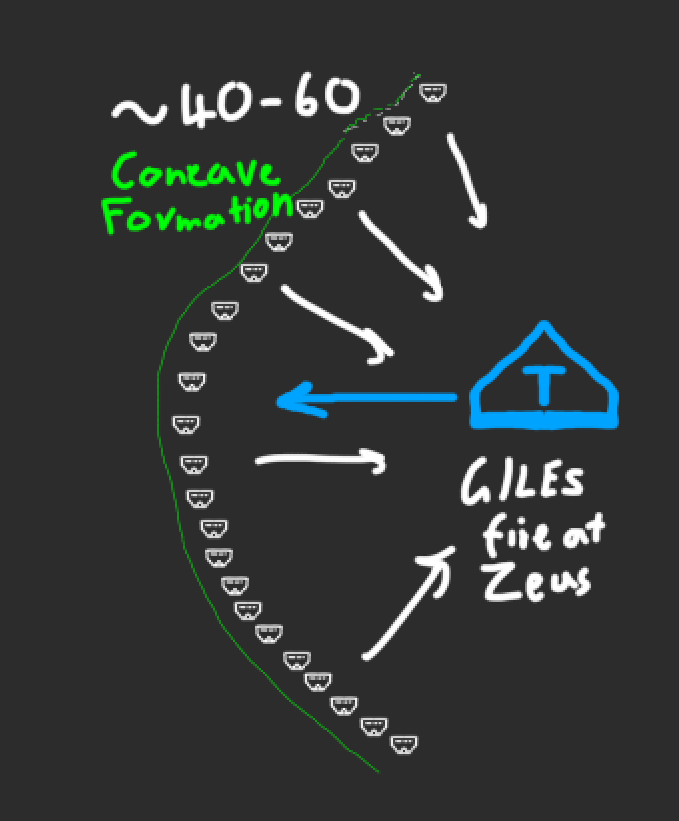
\includegraphics[width=0.7\linewidth]{ODQQ08a}
	\caption{Zeus Titans can be destroyed very easily by Giles, if there is plenty of setup time}
	\label{fig:odqq08a}
\end{figure}

They cannot deal with elevation differences nor can their shots go through base defenses.  


\textbf{Watch out!:} In Vanilla PA games, their shot is a laser that shoot through everything and can't be used to kill air units. 

\textbf{Warning:} These units need lots of care in the presence of an impending army full of fast units.  

\subsubsection{Bluehawks}

Bluehawks are the second long range T2 Bot.  They can attack single targets on sea, land and space.  They are very effective against Atlas titans, all space objects, heavy advance units.  They are weak against swarms of units faster than them.  

\paragraph{Bluehawks and Giles}

These go fantastically together.  The only thing missing is some anti-air and some anti-swarm units.  I normally add slammers to this if need by.  Ratio is 1:1(:1 for slammers), makes for a very versatiles anti-land group.  

Vulnerable to, you guessed it, Shellers.  


\subsubsection{Colonels}
Colonels build the fastest out of any fabricator, has AA, has a very strong anti-mob unit cannon, is weak against strong units and is heavily armored.  It has a huge model footprint and so it is far better to build with an advanced tank fabricator, as they can compress better.  Putting htem into a gruop of advanced bots helps complements the lack of AA.  

They are excellent, I repeat, excellent counters to Zeus.  They are the only land unit capable of putting away significant HP chunks from a Zeus.  


\subsection{T2 Air}


\subsubsection{Phoenix} - If you can't scout other planets effectively, this is the craft to use.  These are invulnerable as they travel through space, getting to the planet.  They are great at removing Zeus titans - provided that you use \textbf{cover the line} mod.  You should protect a zeus with a wing of Phoenixes.  

\subsubsection{Wyrms}  The final word in killing Titans, except for Zeus and Helios titans.  They are slow and vulnerable to everything.  I hate them and only use them if i need to bomb the shit out of one particular unit.  

\subsubsection{Angels} These intercept missiles but do not missiles from sea units, otherwise very useful in late game pushes.   Vulnerable to sea, flak and Giles at the right angle.  

\subsubsection{Hornets}

The advanced bomber is generally a air to ground version of the bluehawk.  It is slow but counters all anti-air buildings and units.  Dies easily to fighters and anti-air land units that move towards it, especially if Giles are present as they counter the missile ammunition fired from the Hornet.  

\subsubsection{Kestrel}

The gunship is great against weak units and is fast and hardy enough to deal with a commander.  About 20-25 are required to kill a commander.  Vulnerable to flak, fighters.  Combine with Phoenix for an excellent fast moving attack group.  Combine that group with Arngels and Hornets for a force to kill land units.  

\subsubsection{Horsefly} 

I really don't get this unit.  It's literally a dox that flies and has lots of armor.  It has a bit of DPS but is fairly expensive.  

\subsection{Air transports}

Strategies involving tanks benefit from air transports.  Moving combat fabricators around also helps in setting up teleports.  

\begin{figure}[h]
	\centering
	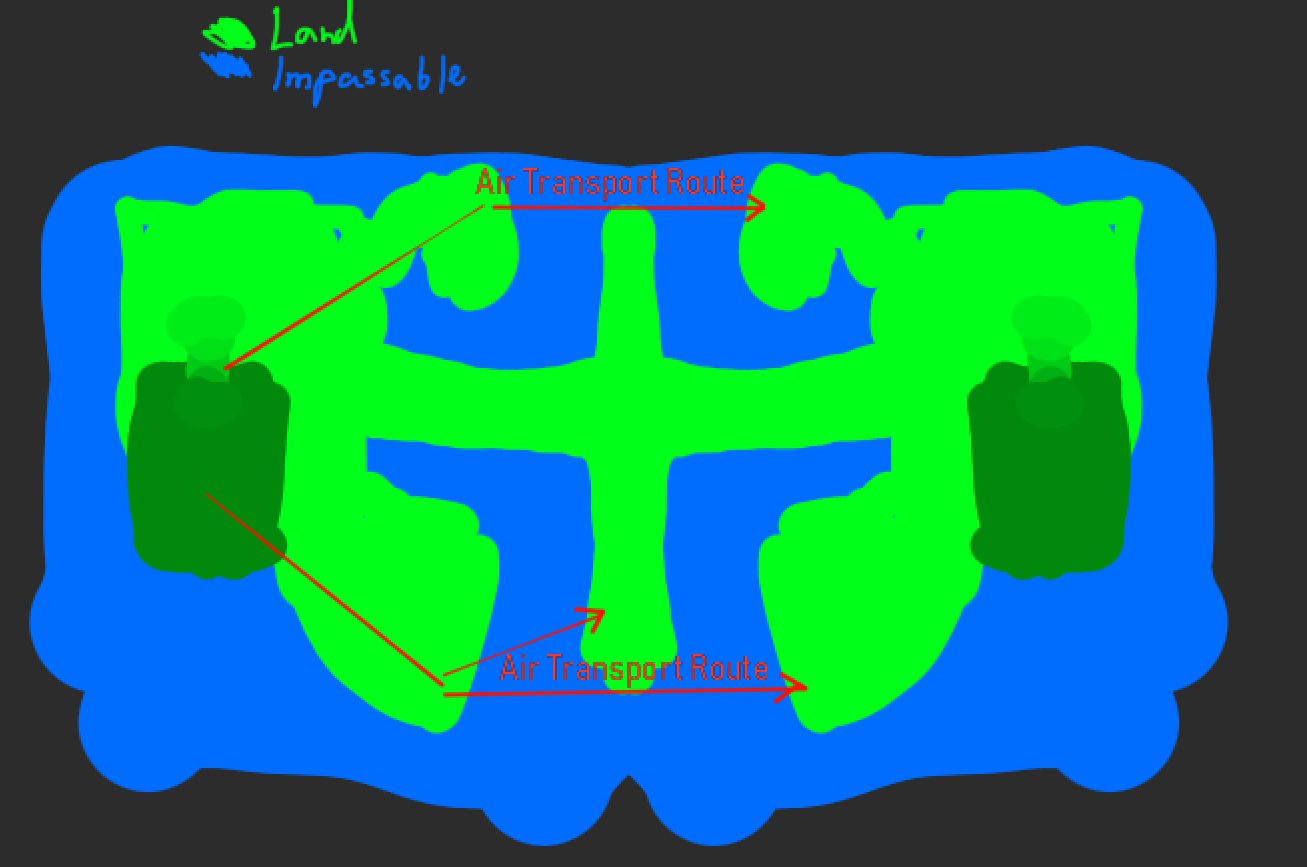
\includegraphics[width=1\linewidth]{k65pOTe}
	\caption{Air Transports open up different routes - if you can control the air}
	\label{fig:k65pote}
\end{figure}


Dropping 5-10 levellers on an undefended base with a commander in it is ultimately the end of that game.  

\textbf{Protip:}  You can't pick up your commander with a pelican.  At all.  

\subsubsection{Sneaky Teleport}

Doing this with a combat fabricator is cheap and fast.  You pick up 1 or more combat fabs and scout the future landing spot, find a vulnerable path and quickly build a teleport for your forces to flank an enemy base right in the weakspot

\textbf{Author's Note:}  I have done this only a handful of times when the time called for it and it's moments like those that have to be treasured by watching the post-game replay and observing mass ping spam reactions, entire armies being routed as bases and economies are set ablaze and devastated.  

\newpage
\section{Commander Strategies}  

Commanders are very useful units and like many commanders in other Annihilation games, they form the cornerstone of your early game strategy.  

\subsection{Offensive}

The most ballsiest move I can ever describe in early game is pushing your commander forward into the front.  It is, quite simply, a power move of astronomic proportions and incredibly risky.  With no radar, boombots become your biggest threat.  With no energy, you have no dgun/ubercannon with which to dispatch the enemy hordes.  

This is most applicable on small maps with metal located away from the start area.  

I have had allies watch me do this and react with pings and disapproval.  It forces your allies to do play offensively as well as it can be partially inspiring.  

\subsubsection{Commander Pushing}
\label{commpush}
\begin{figure}[htb]
	\centering
	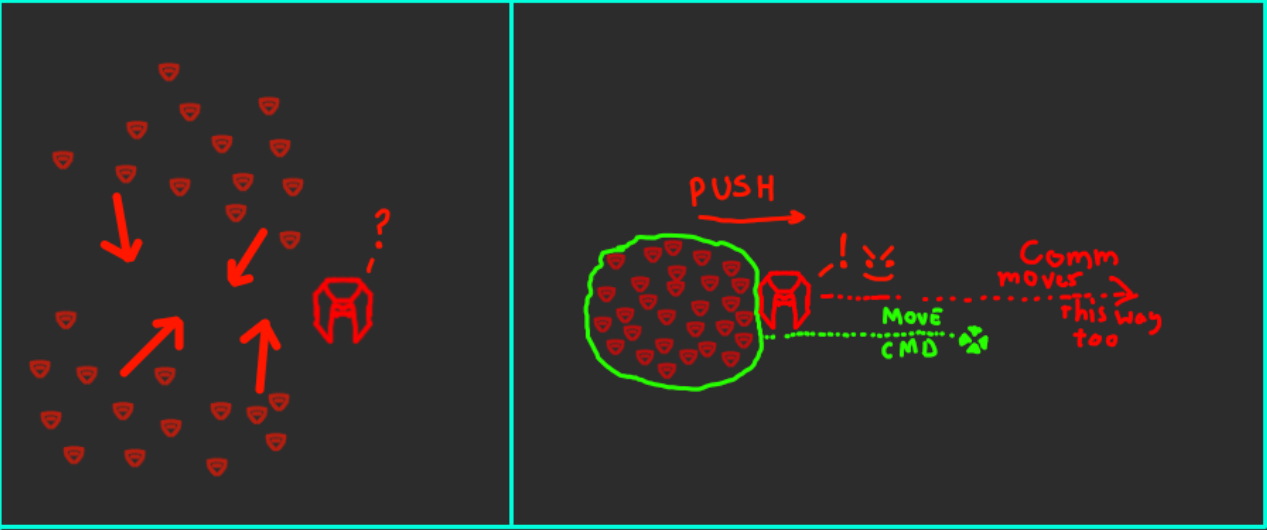
\includegraphics[width=\linewidth]{uyhiwZs}
	\caption{Pushing a commander using Dox}
	\label{fig:uyhiwzs}
\end{figure}
This is where you get a bunch of units, which are faster than a commander, to push it.  One important move command is ctrl right mouse click.  This is really only viable in early game and you can push your commander right up to another player's area.  This can be a powerful blocker against whatever.  
\subsection{Defensive}

Keeping the commander at base is what happens in most situations.  The Dgun/Ubercannon is fantastic against small incursions.  The commander becomes more of a liability as time goes on, as many of you, who are reading this, would know.

\subsubsection{Anti-space}

It is somewhat little known that the Omega battleship cannot hit the commander if it is entirely underwater.  Everything else can.  



\subsection{Next world expansion}

Commanders can be used to build an expansion base and quickly setup a few factories.  However, if the planet is occupied, the occupier might not like your presence and will commit to killing your comm or worse, expel you from the planet.  

\section{Psychological Warfare}\label{sec:psychological-warfare}

Probably one of the few aspects of the game that is talked about with other players I find is the psychological warfare that is unleashed by players on other players.  

Not the same as attention warfare described in \ref{sec:attention-warfare}

\subsection{Invasion (On Ground)}

Seperated or not from section \ref{sec:massive-army}, a ground invasion of a planet is the most important thing to repel.  It also draws the sudden attention \ref{sec:attention-warfare} of the enemy and possibly their team mates with pings being spammed.  

For the defender, it is vitally important a ground invasion is dispatched.  For the offender, you have to ensure it survives in whatever form it needs to be.  




\subsection{Massive Army}\label{sec:massive-army}

Fewer things in the game make a player reel harder than an overwhelming force. Its far worse just by looking at it.  

These things are one of the few use cases for a Nuclear missile, although you have to calculate if it is worth the 30k metal.  You also have to anticipate the landing spot of said nuke.  

There is no mobile anti-nuke in PA and therefore the task that falls to you is to split your forces up so that you will have to eat several nukes in order to have your army be totally destroyed.  This requires more of your attention and more actions per minute, but considering how slow a tank army moves, this can be done with ease.  

A t1 bot army is a little harder to do in this case, but they should really be set on global patrol from a teleporter anyway, in most general cases.  

\subsubsection{Global invasion}

The massive army is a bad thing to see.  What is worse, is a teleport set to global patrol instead of a move waypoint with hundreds of fast moving units flowing out of it going in every direction possible.  In seconds, you have units flying everywhere and if not prepared, you will lose your economy very quickly and will have to rely on metal storage.  This is not a game ending strategy but could be if not handled correctly swiftly.  If combined with the massive army, the boombots or locusts would be the first wave and the second one will be tanks, perhaps taking out resistance hotspots as a group.  

To the unprepared, this drains the morale of any player, especially those who know the ramifications that their planet is suddenly no longer theirs.  

To defend against this, air units are needed.  Alot of gunships are using the mod \textbf{cover the line (now part of the game[Maybe])}. 


\begin{figure}[h]
	\centering
	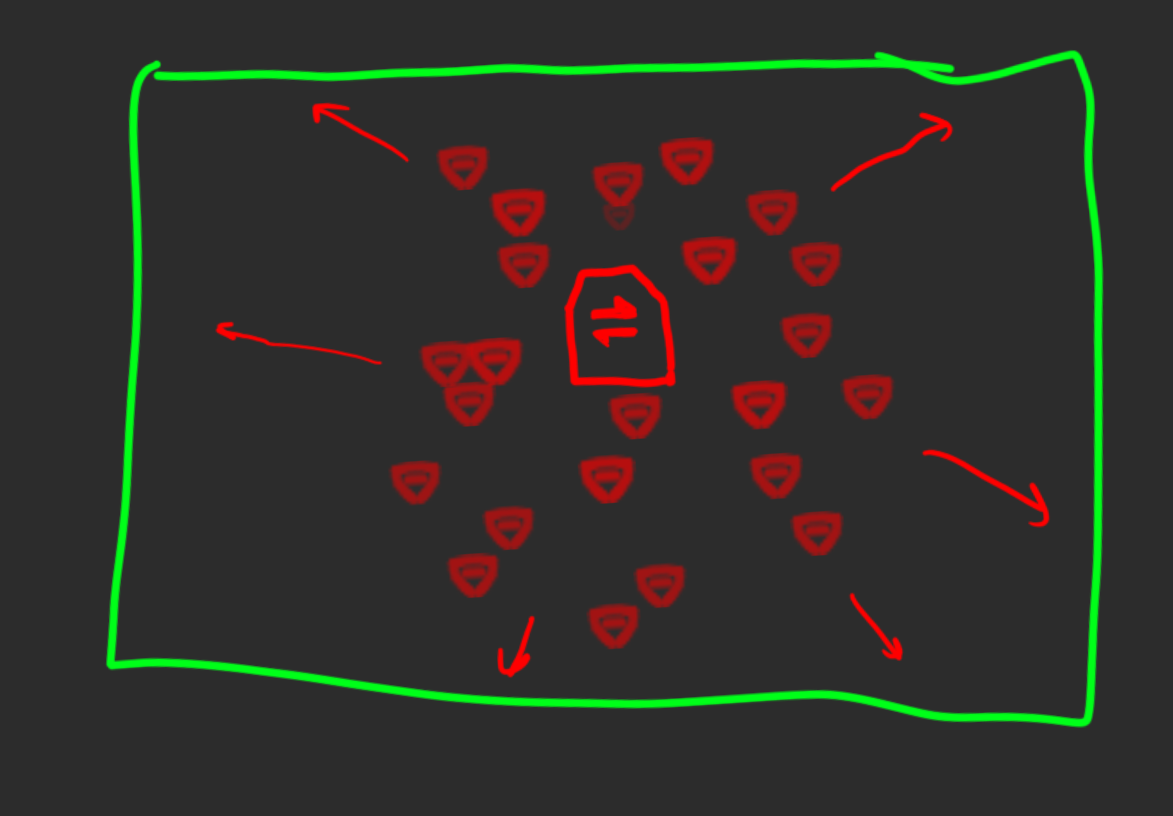
\includegraphics[width=0.7\linewidth]{mYZYLlR}
	\caption{A global invasion will look roughly like this, just add in your opponents economy buildings and perhaps a very salty response.  Locusts work well here as well}
	\label{fig:myzyllr}
\end{figure}



\subsection{Losing Gas}
\label{sec:losing-gas}

The gas planet in games is seen as the king of resources.  If you take it, you have all the resources in the world.  Or the universe.   Whatever.  

If you lose it, whatever you were doing is now ruined.  Losing it could present you with a rapidly limited choice of options and one of them could be firing off the 30 nukes that have been stockpiled.  

Losing gas is most often done using Artemis railgun units.  These can kill Jigs at long range without dying to the explosion.  These can be countered with avengers or, considering that having gas means you have the means to do it, attack the enemy's space production building these ships.  It can only be done in space.

\subsection{Getting Pinned}


Getting pinned is awful, see section \ref{subsec:pinning}.  It may be in your interest to just maintain a pin and attack piecemeal whilst attacking another player, because the pinned player might just give up, disconnect or self destruct, saving you losing an entire attack force to killing the commander.  





\subsection{Mass Fabricator invasion}

Invading with a metric shit ton of fabricators requires a relatively safe teleporter location.  This can be used to build a quick anti nuke and/or several titans. Requires lots of metal for whatever you need to do.  A player that sees a fabricator swarm rather than an army should assume alot of things could happen and should move to destroy them as quickly as possible.

Space fabricator invasions are also quite deadly as they can build (with enough available metal) titans with ease.    

\subsubsection{Ragnarok}
The subset of the Mass Fab Invasion.  

Ahh the Ragnarok.  It elicits a picture of massive economic destruction that drives many players to press shift-f7, attack move to that spot and then press shift-f9 to the area.  If this fails, the game is over for some.  

This is an option if you cannot pay attention to that planet and your focus is on things else where.  
\newpage
\section{Ping pathing}

In PA, there is absolutely no way to describe an attack path, which can describe where .  The only way to do this is to do it using ping spam.  Default key for it is 'G' on latin keyboards.  Holding down 'shift' after pressing 'G' will allow you to spam pings.  

The bad side of doing this is that some players have no idea whats going on or don't have the reaction time to read the situation and just get annoyed. 

\textbf{Author's note:} Longer Pings by Captain Conundrum is a mod that makes pings last longer and can be very useful.  


\section{Appendix: Glossary}

Teleports - Gates, Stargates, Teleporters all are interchangeable but I have tried to keep it to teleporters.  These require energy to move units from one place to another.  

\end{document}
